% !TEX root = ../partial-sdm.tex

\chapter{Results (v): Supervised classification application}

Supervised classification problem consists of categorize data into groups after seeing some samples from each group. First, it is presented pieces of data with their categories. The algorithm learns from these data, which is known as learning phase. Then, new pieces of data are presented and the algorithm must classify them into the already known groups. It is named supervised because  the algorithm will not create the groups itself. It will learn the groups from during the learning phase, in which the groups have already been defined and the pieces of data have already been classified into them.

Although this problem has already been studied (REF), our intention here is to show that a pure SDM may also be used to classify data. \citet{fan1997genetic} has used SDM to solve a classification problem, recognizing handwriting letters from images, but he used a mix of genetic algorithm with SDM, which is very different from the original SDM described by \cite{Kanerva1988}. Even though his algorithm has classified properly, we were intrigued whether a pure SDM would also classify successfully.

Hence, we have developed a supervised classification algorithm based on a pure SDM as our main memory. Our goal was to classify noisy images into their respective letters (case sensitive) and numbers. For some examples, see Figure \ref{fig-classification-examples}.

\begin{figure}[!htb]
\centering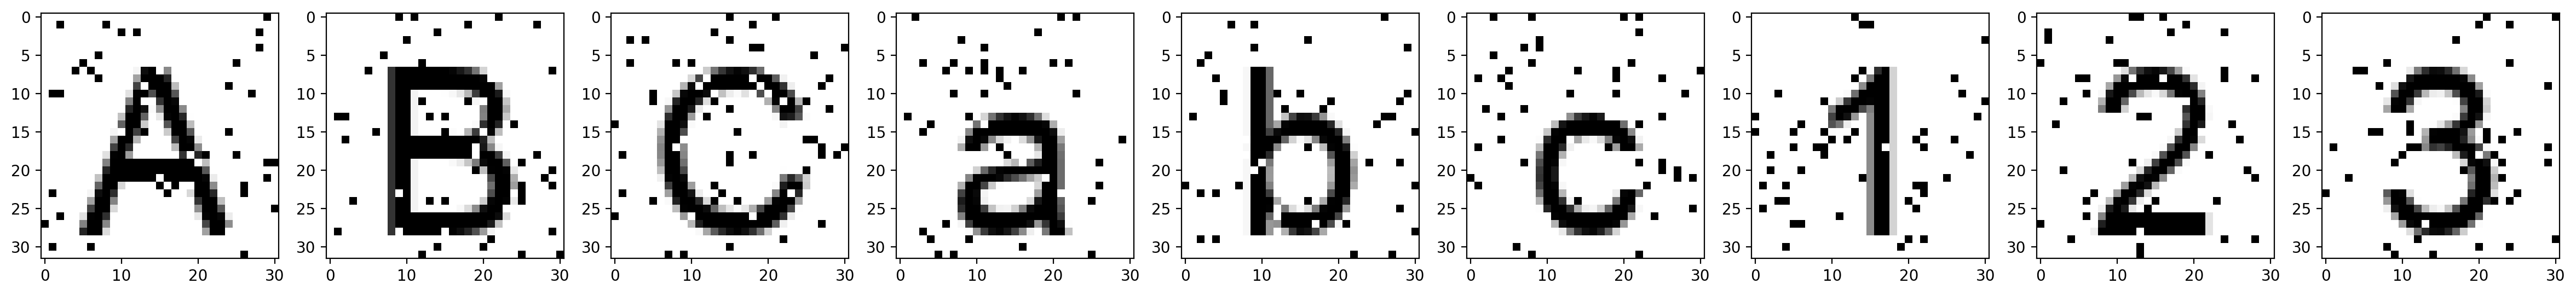
\includegraphics[width=\textwidth]{./images02/classification/example.png}
\caption{Examples of noisy images with uppercase letters, lowercase letters and numbers.
\label{fig-classification-examples}}
\end{figure}

The images had 31 pixels of width and 32 pixels of height, totaling 992 pixels per image. Each image was mapped into a 1,000 bit bitstring in which the bits were set according to the color of each pixel of the image. So, white pixels were equal to bit 0, and black pixels to bit 1. The 8 remaining bits were all set to zero. This was a bijective mapping (or one-to-one mapping), i.e., there was only one bitstring for each image, and there was only one image for each bitstring.

% TODO Add image showing the association between pixels and bits.

A total of 62 classification groups have been trained in the SDM. For each of them, it was generated a random bitstring. Thus, the groups' bitstrings were orthogonal between any two of them. There is one image for each of the 62 groups in Figure \ref{fig-classification-groups}. Notice that the SDM has never seen a single image with no noise.

\begin{figure}[!htb]
\centering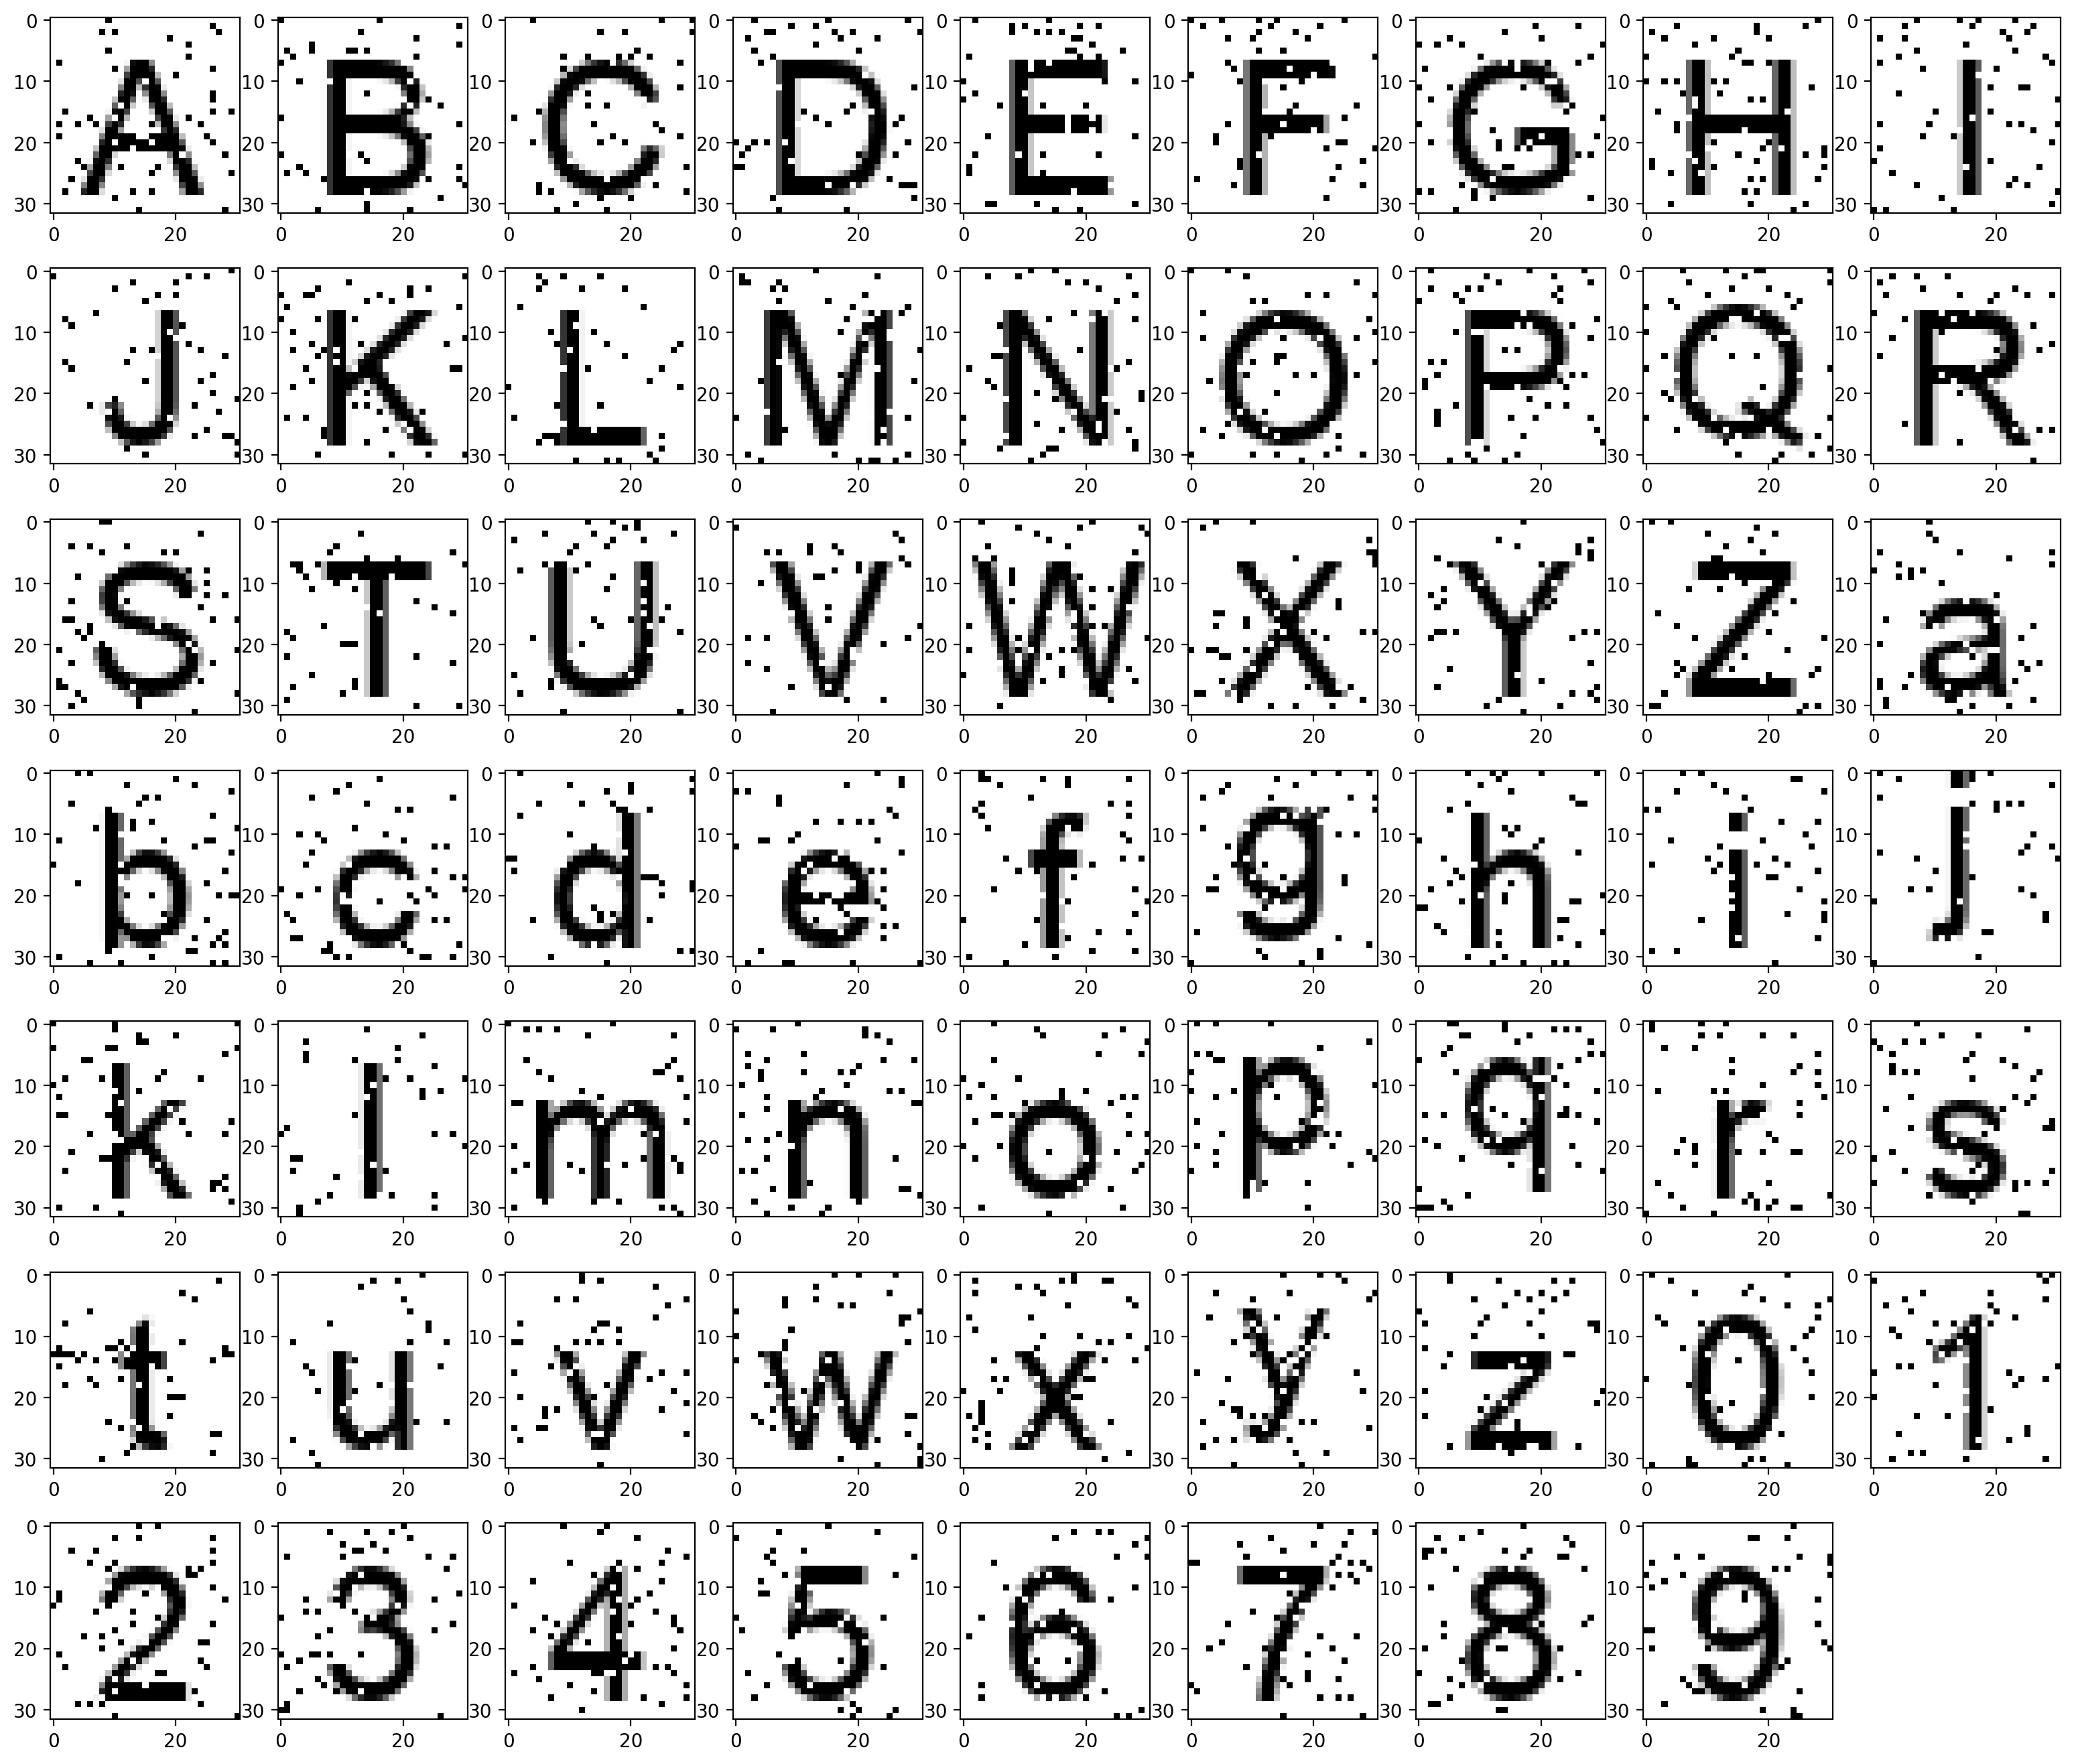
\includegraphics[width=\textwidth]{./images02/classification/groups.png}
\caption{One noisy image for each of the 62 classification groups.
\label{fig-classification-groups}}
\end{figure}

The association of images to groups was stored as sequences in SDM, as detailed by \citet{Kanerva1988} in Chapter 8. During the learning phase, the image bitstrings were stored pointing to their groups bitstrings, i.e., write(addr=bs\_image, datum=bs\_label). Thus, in order to classify an unknown image, we only had to read from its address and check which group has been found.

% TODO Add image showing the pointers.

During the learning phase, we have generated 100 noisy images for each character. The images had 5\% of noise, i.e., 5\% of their pixels have been randomly flipped. For example, see the generated images for letter A in Figure \ref{fig-classification-training-A}. Then, we have wrote the classification group bitstring into the bitstring associated to each noisy image, i.e., write(bs\_image, bs\_label). For a complete image training set, see Appendix XYZ.

\begin{figure}[!htb]
\centering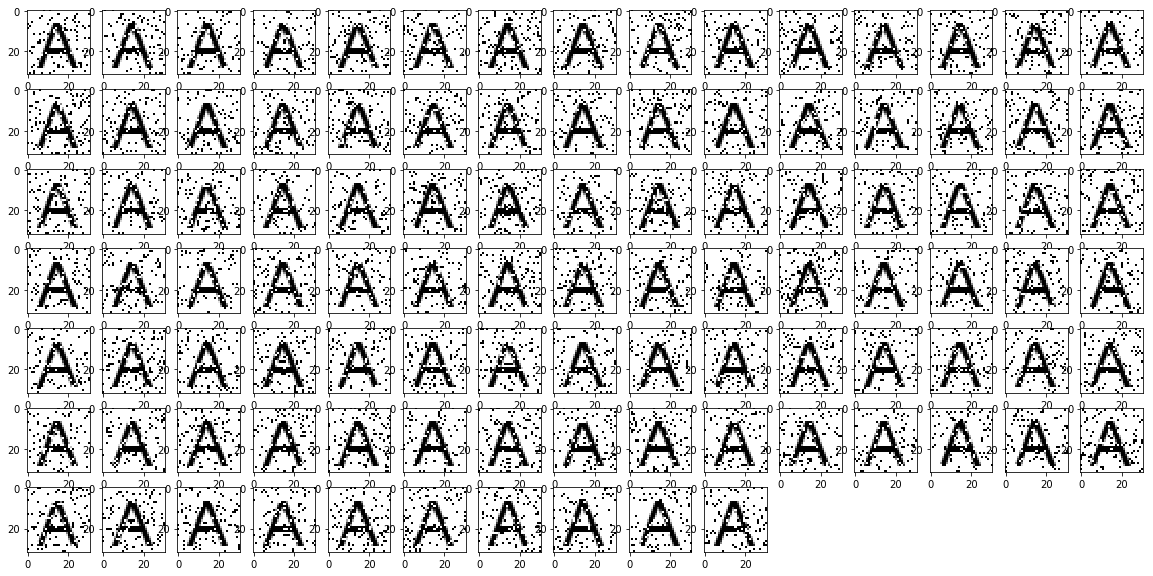
\includegraphics[width=\textwidth]{./images02/classification/trainingA.png}
\caption{100 noisy images generated to train label A.
\label{fig-classification-training-A}}
\end{figure}

Finally, we have assess the performance of our classifier. We had done it in three different scenarios: high noise (20\%), low noise (5\%) and no noise. See Figures \ref{fig-classification-noise-high} and \ref{fig-classification-no-noise} for images with 20\% noise and no noise. The low noise scenario had the same noise as the training set. For each scenario, we had classified 620 unknown images with 10 images per group.

\begin{figure}[!htb]
\centering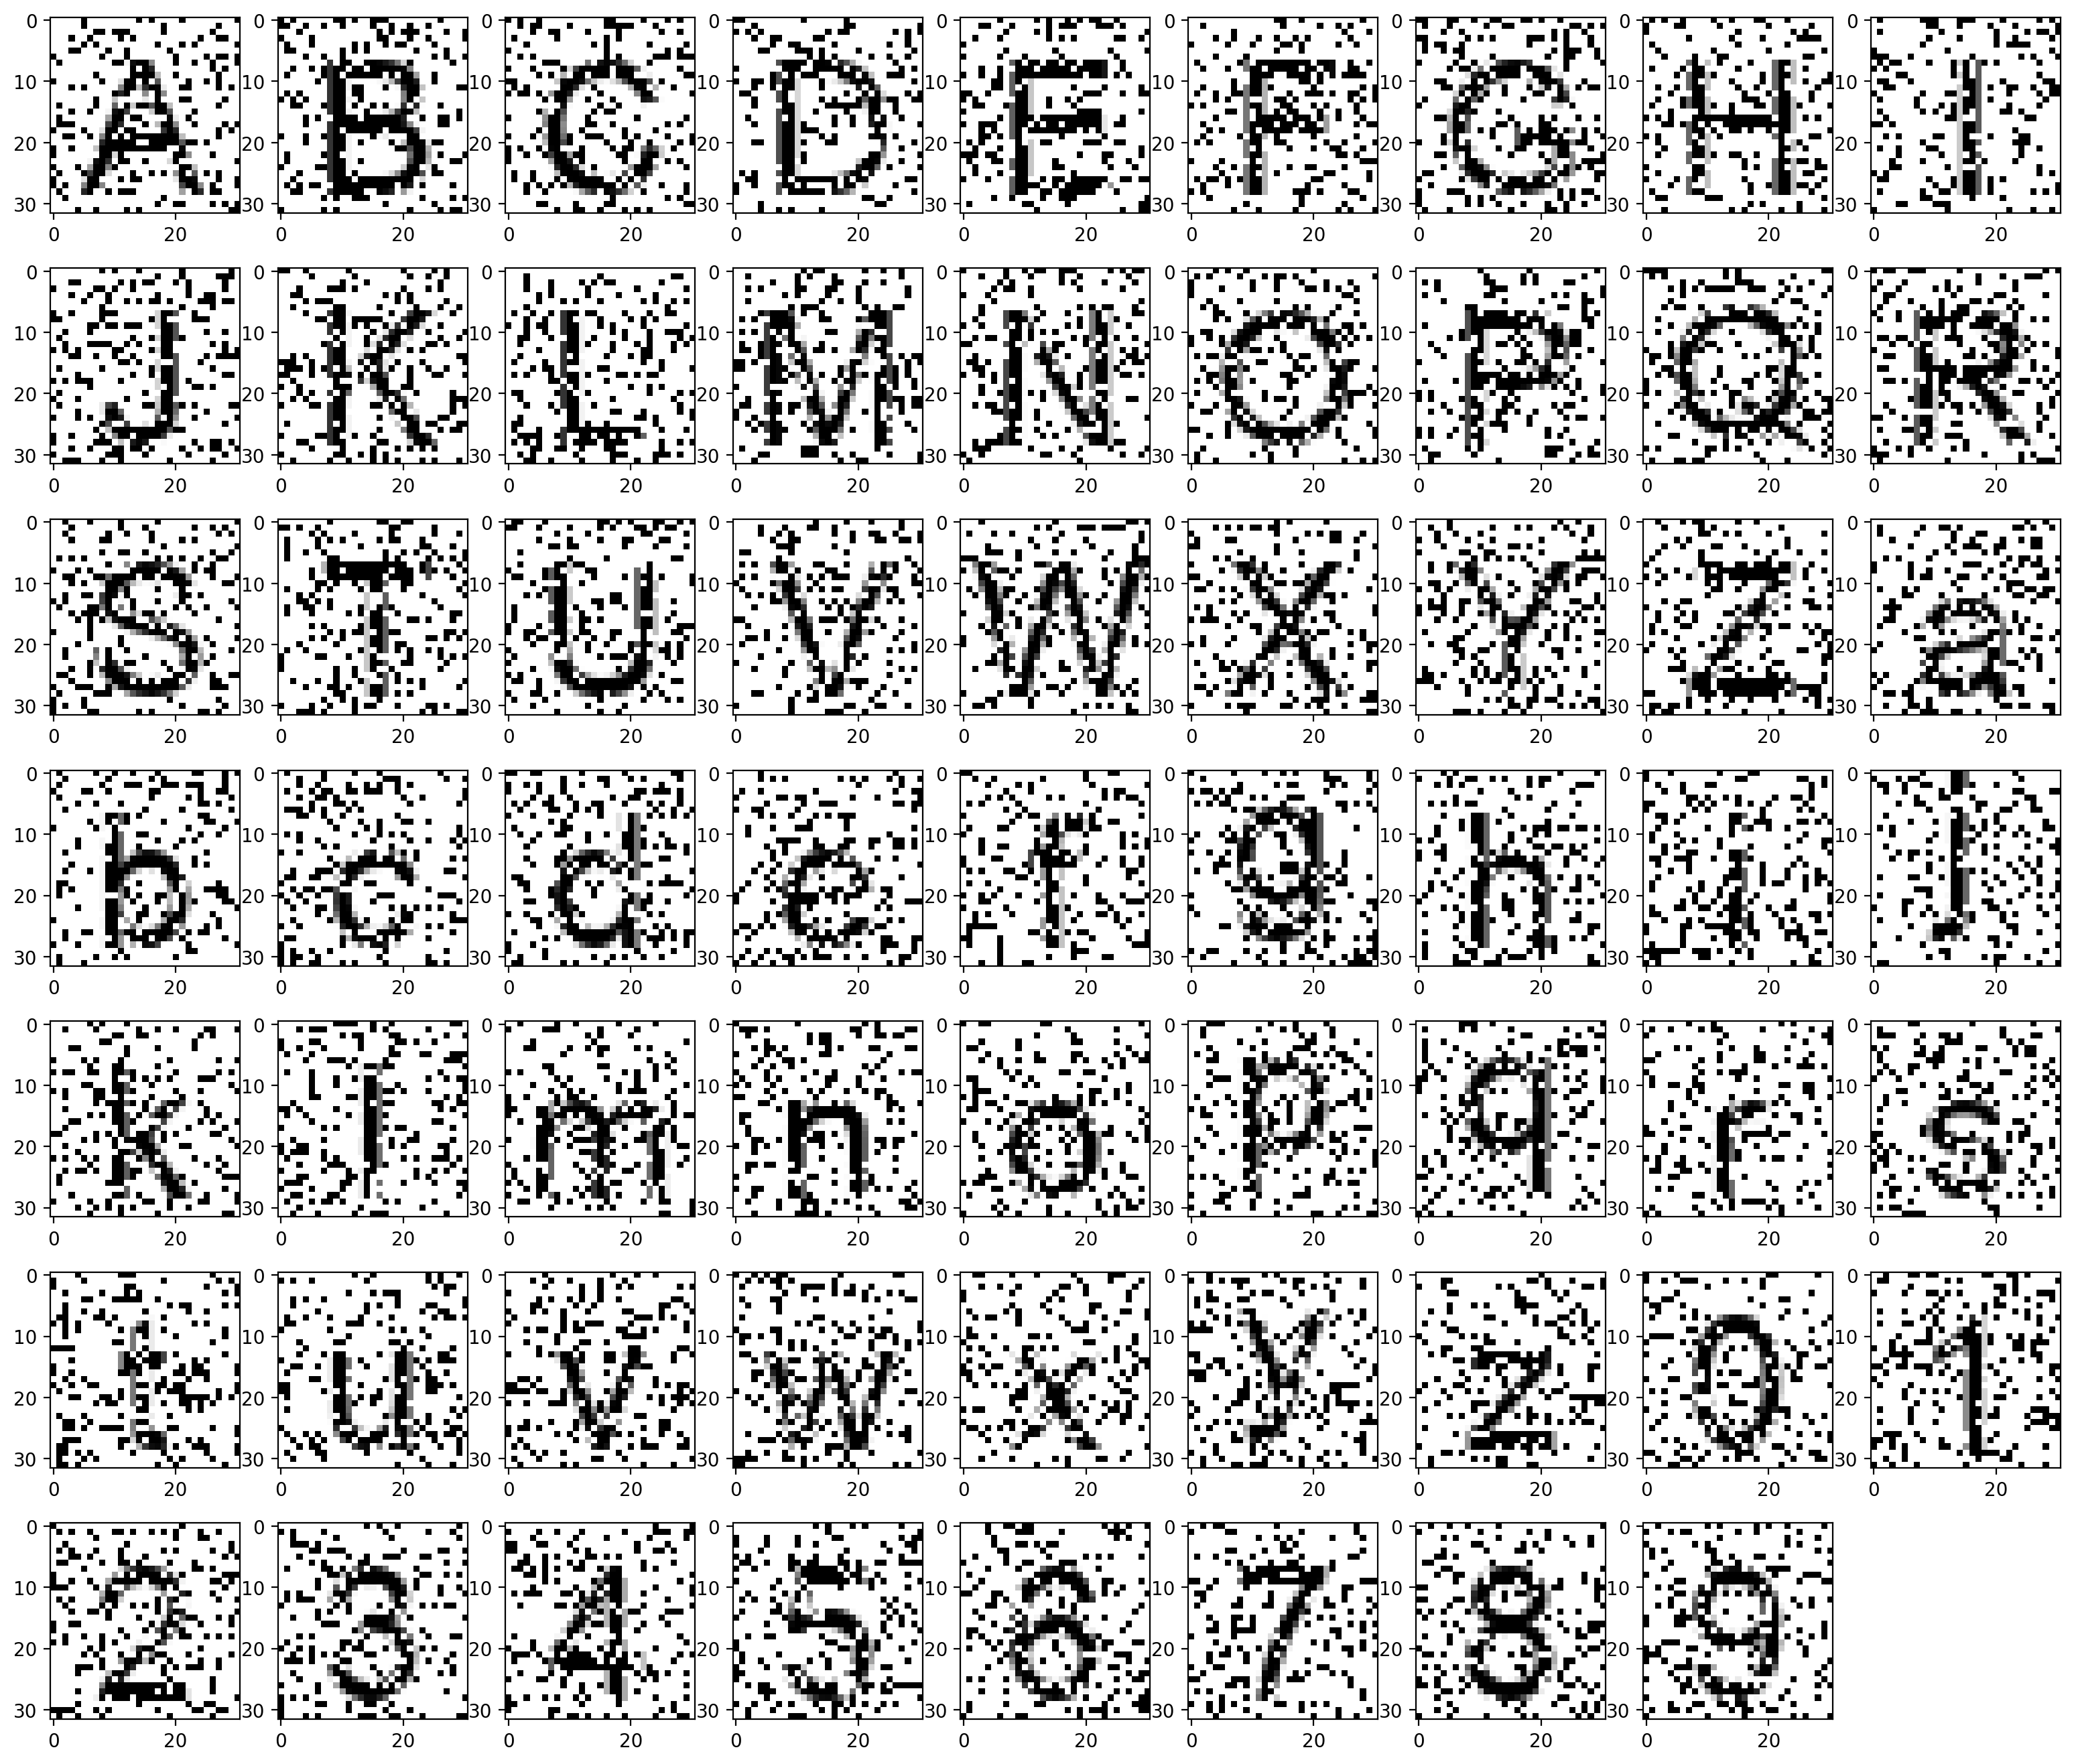
\includegraphics[width=0.75\textwidth]{./images02/classification/noise-high.png}
\caption{Images generated using a 20\% noise for the high noise scenario.
\label{fig-classification-noise-high}}
\end{figure}

\begin{figure}[!htb]
\centering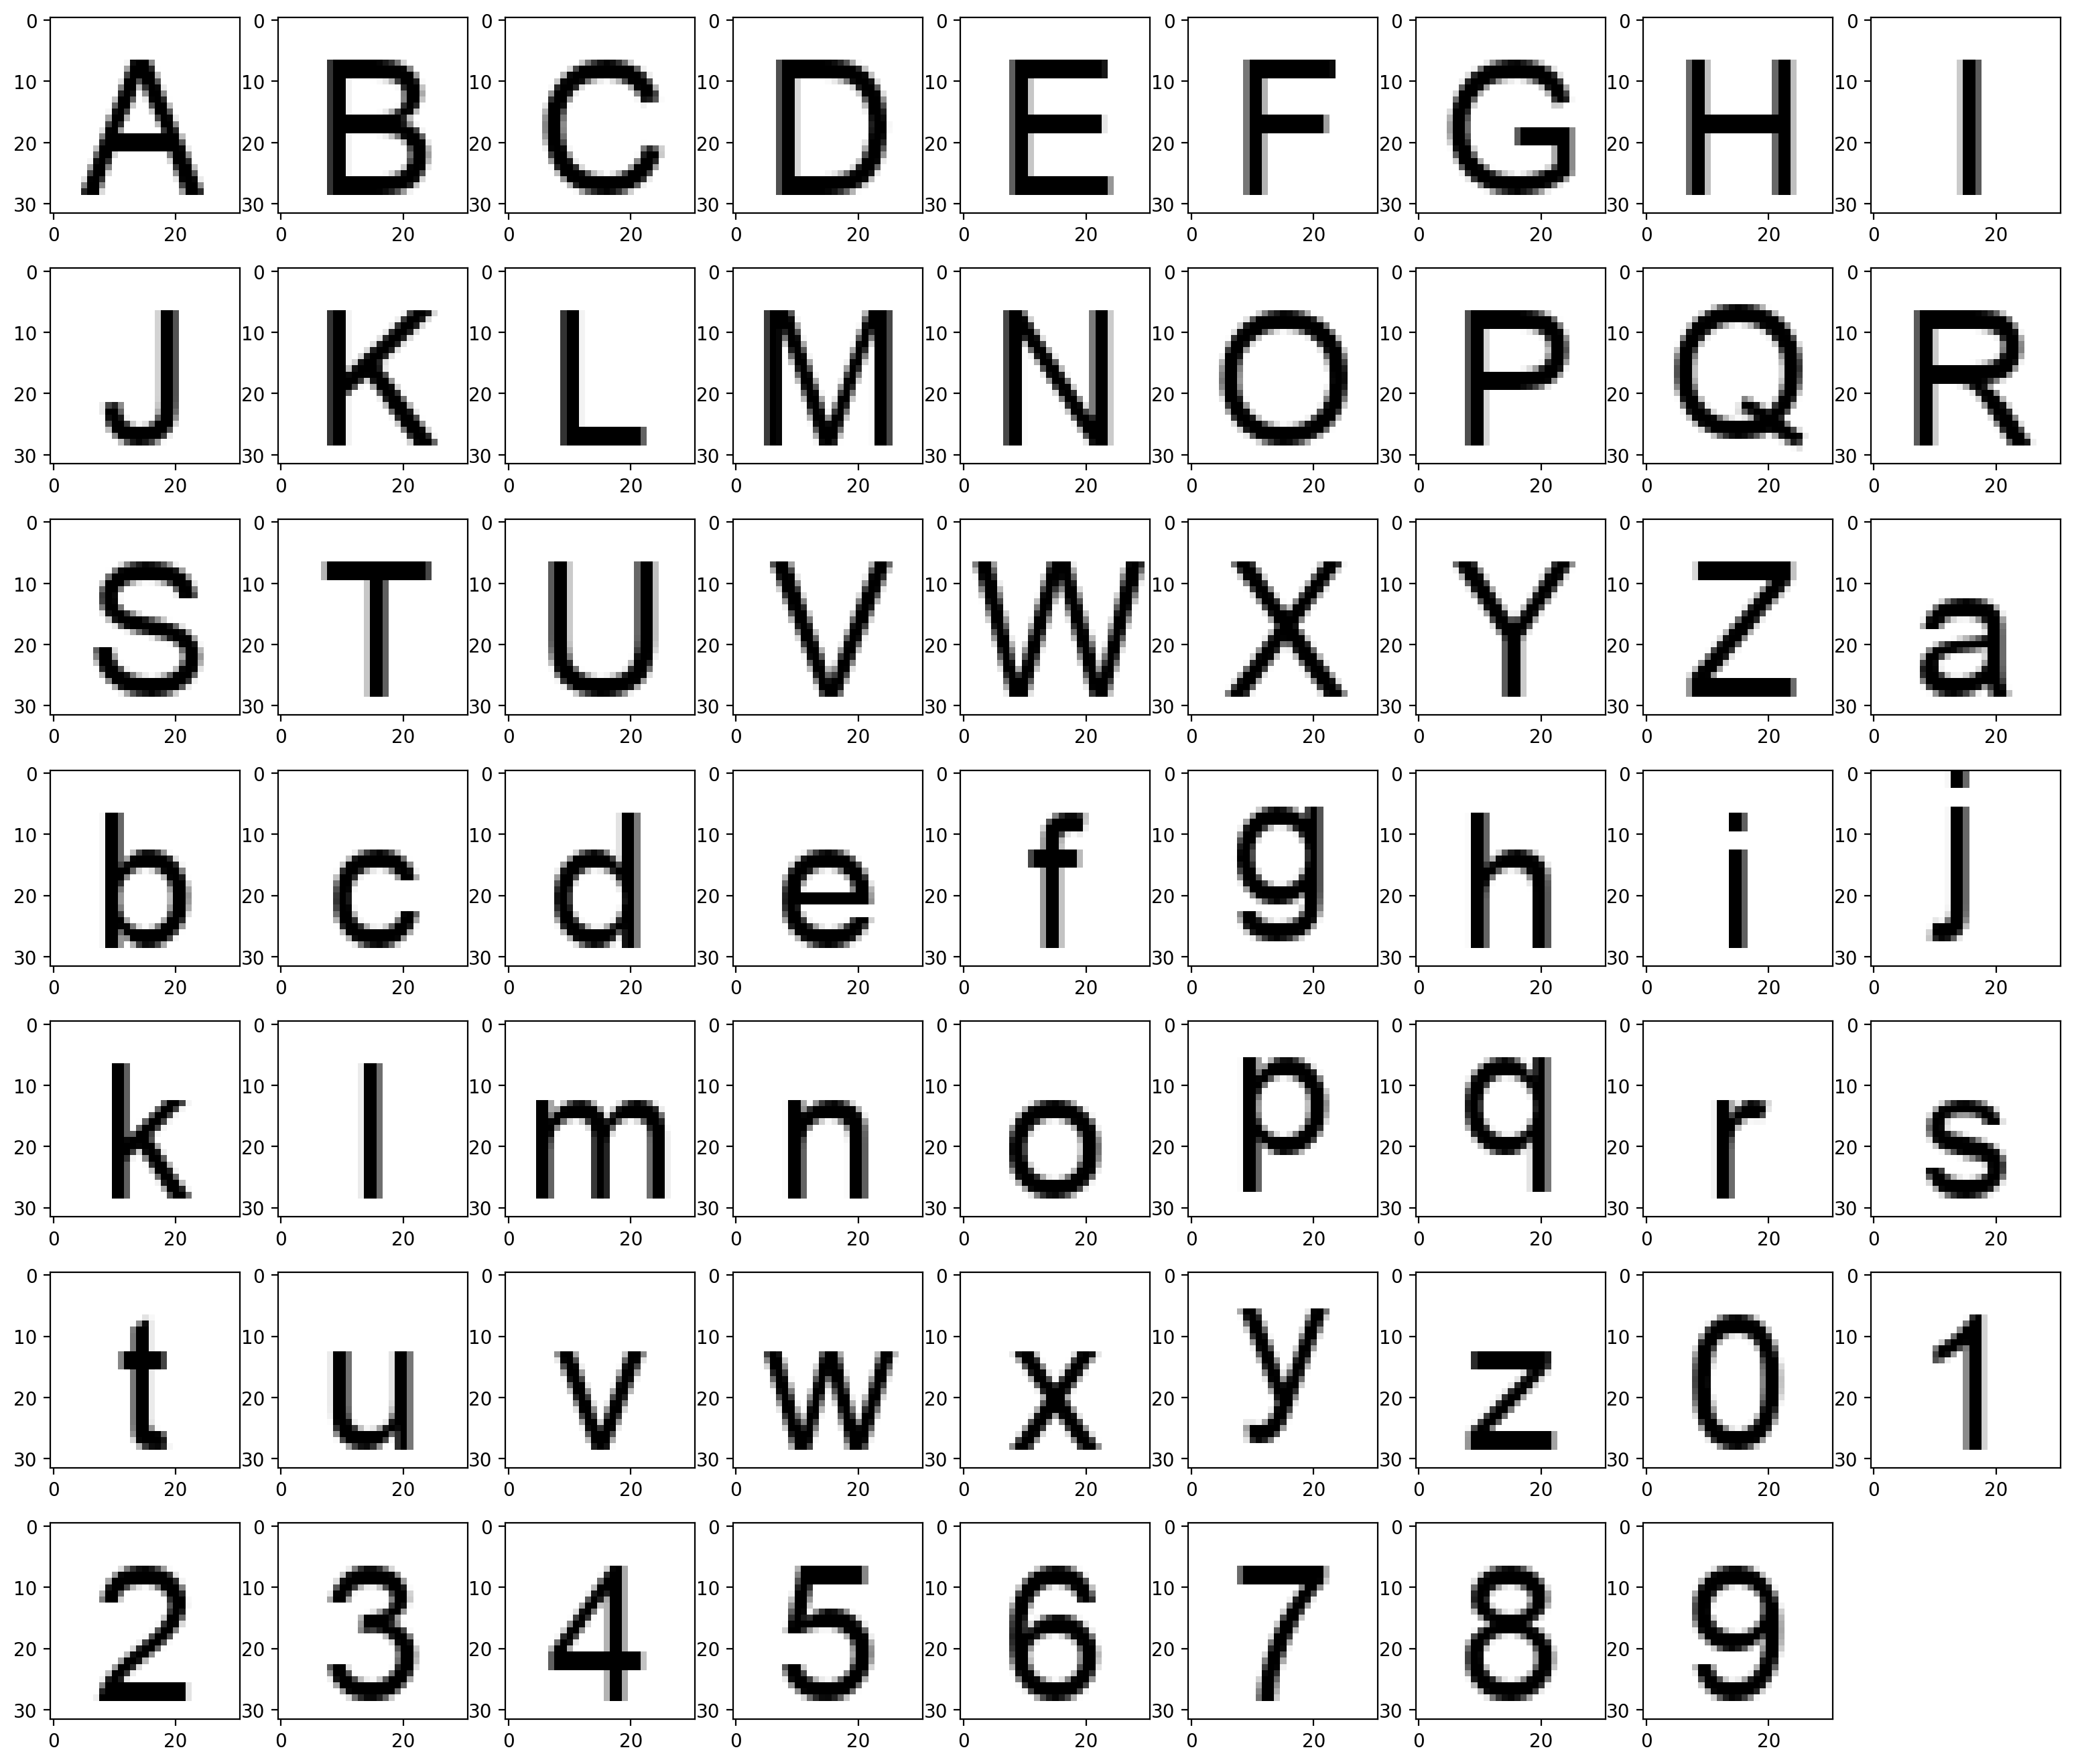
\includegraphics[width=0.75\textwidth]{./images02/classification/no-noise.png}
\caption{Images generated for the no noise scenario.
\label{fig-classification-no-noise}}
\end{figure}

The performance was calculated as the percentage of hits for each group. We did not expected the same performance for all groups because some groups become very similar to other depending on the noise level, and this similarity may even confuse a person (see Figure \ref{fig-classification-similarity}).

\begin{figure}[!htb]
  \centering
  \subfloat[``i'', ``l'', and ``r'' with 20\% noise.]{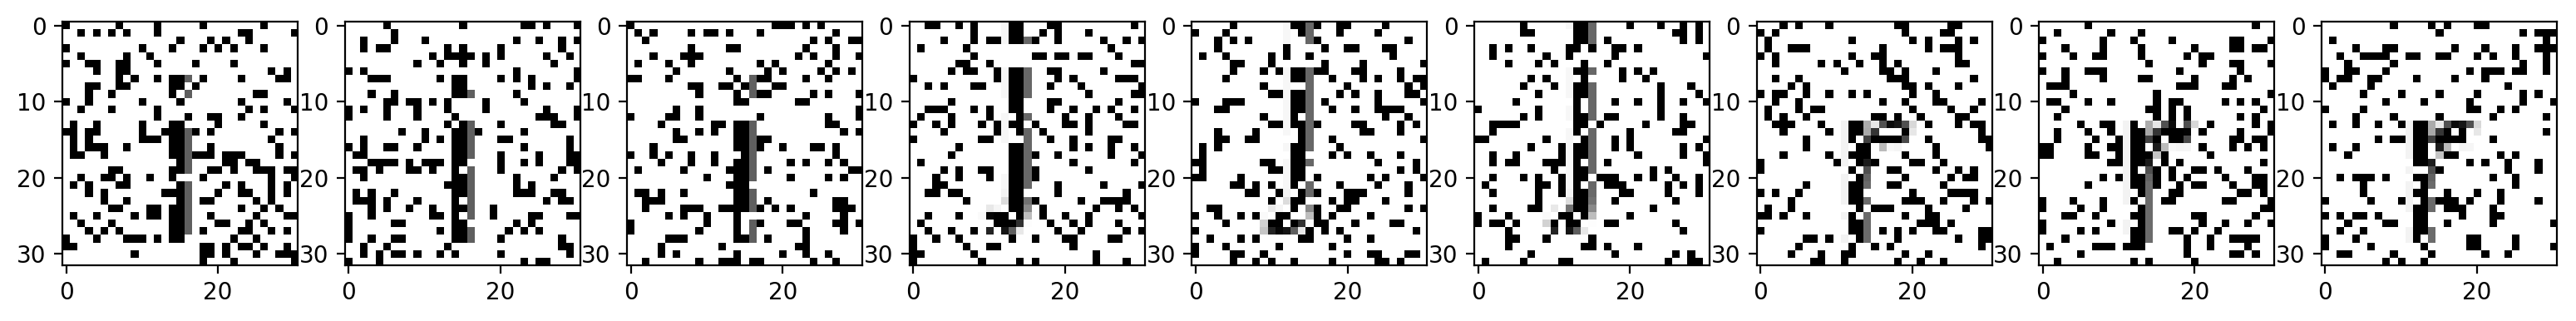
\includegraphics[width=\textwidth]{./images02/classification/ilr-high-noise.png}}

  \subfloat[``i'', ``l'', and ``r'' with 5\% noise.]{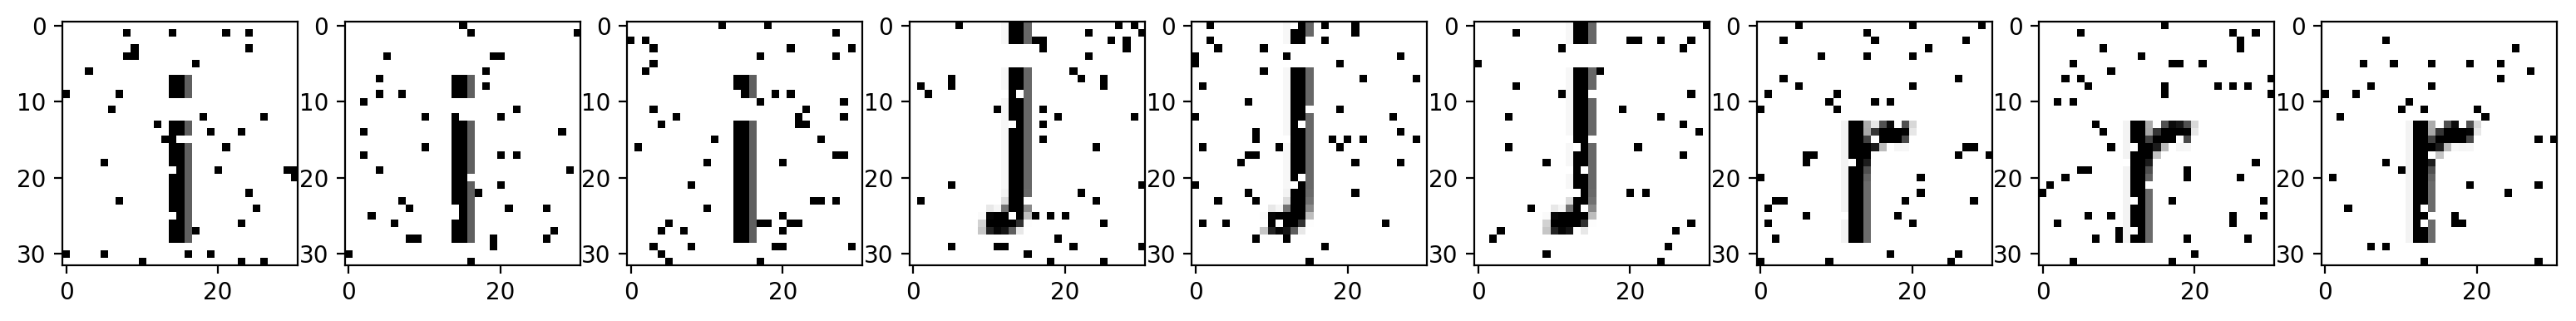
\includegraphics[width=\textwidth]{./images02/classification/ilr-low-noise.png}}

  \subfloat[``c'', ``d'', and ``o'' with 20\% noise.]{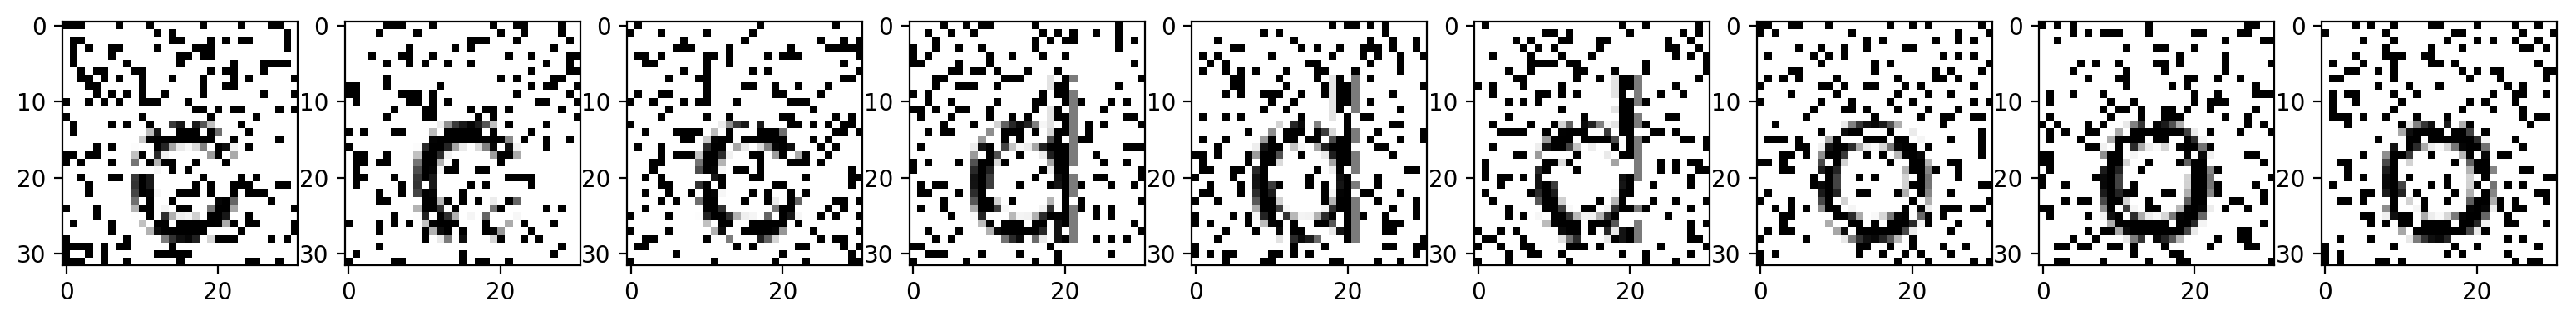
\includegraphics[width=\textwidth]{./images02/classification/cdo-high-noise.png}}

  \subfloat[``c'', ``d'', and ``o'' with 5\% noise.]{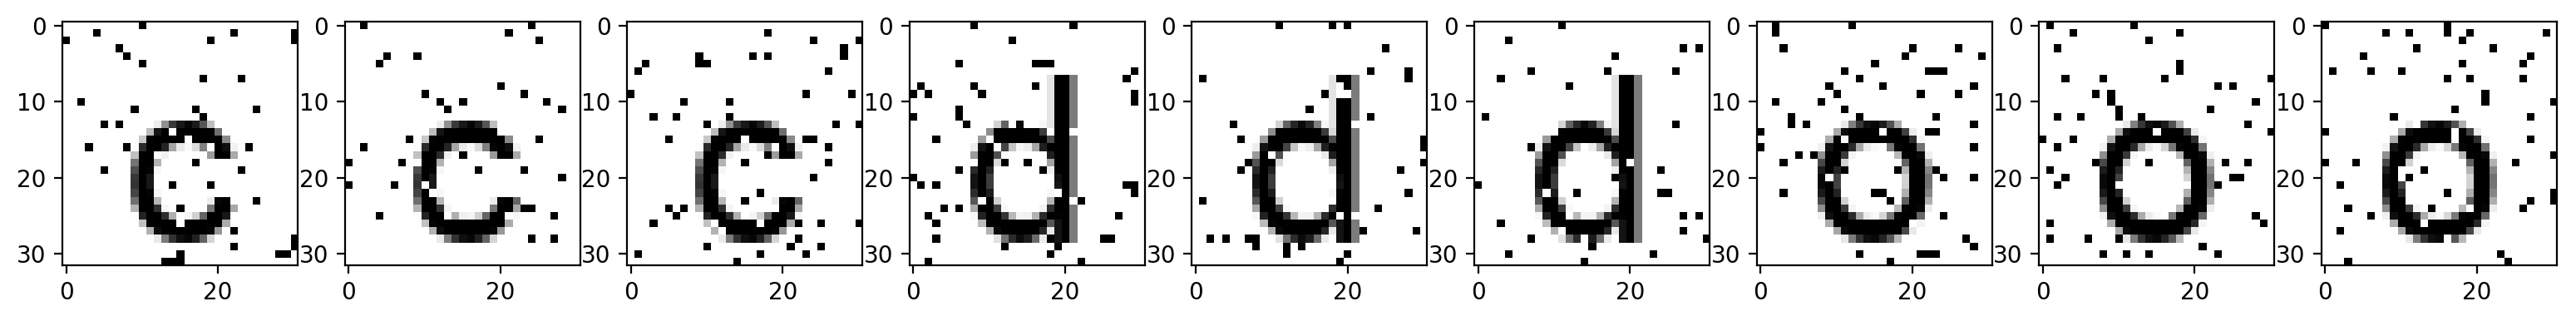
\includegraphics[width=\textwidth]{./images02/classification/cdo-low-noise.png}}

  \subfloat[``G'', ``O'', and ``Q'' with 20\% noise.]{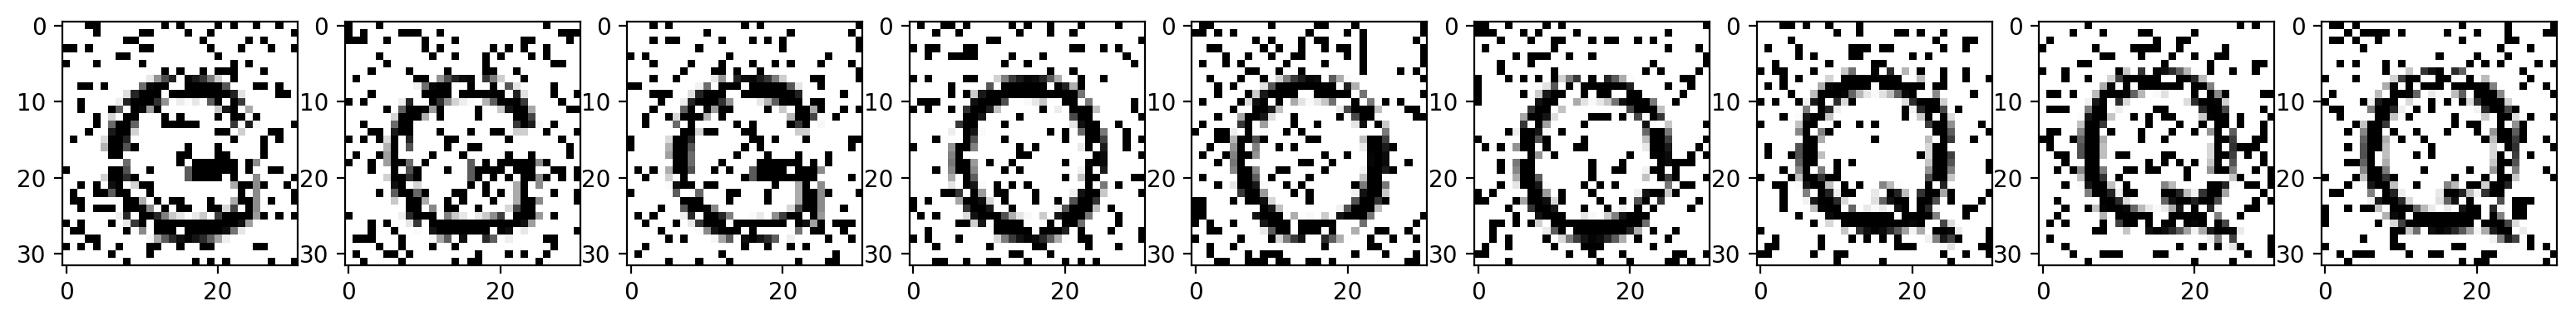
\includegraphics[width=\textwidth]{./images02/classification/GOQ-high-noise.png}}

  \subfloat[``G'', ``O'', and ``Q'' with 5\% noise.]{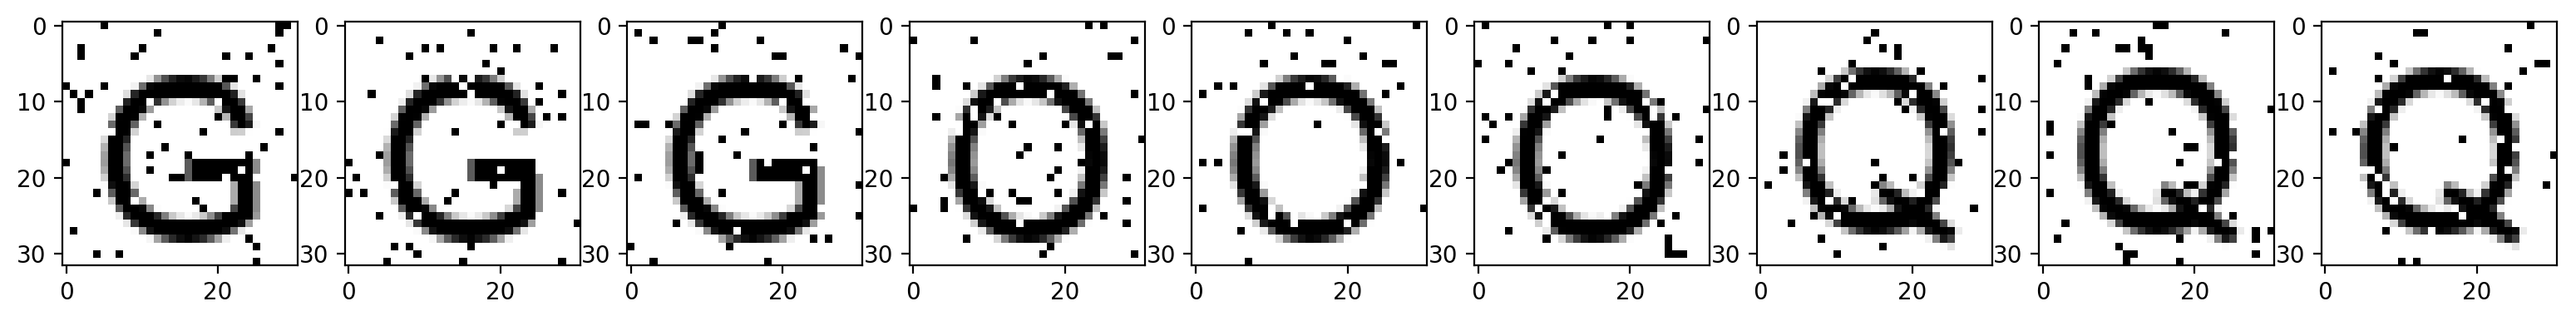
\includegraphics[width=\textwidth]{./images02/classification/GOQ-low-noise.png}}

  \caption{Images of different characters which may be confusing depending on the noise level.}
  \label{fig-classification-similarity}
\end{figure}

In the no noise scenario, the classifier has hit all characters, except letter ``l'' which was wrongly associated to the group of ``i''. We believe that it happened because the classifier had never seen an image with no noise and the difference between the images of ``l'' and ``i'' is smaller than the critical distance. So, both groups have been merged and it would converge to only one of them. In our simulation, it happened to be the group of ``i''.

In the low noise scenario, it has made few mistakes. It correctly classified all images but some from characters ``b'', ``e'', ``f'', ``l'', ``t'', and ``9''. It completely classified ``l'' images to the ``i'' group. In the other cases, it made just a few mistakes. See Figure \ref{fig-classification-low-noise-results} to check the images and their classification.

\begin{figure}[!htb]
  \centering
  \subfloat[Images from character ``b which were classified as {[b, b, b, h, b, o, b, h, b, b]}, respectively. It has made 3 misses.]{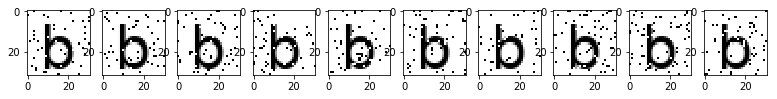
\includegraphics[width=\textwidth]{./images02/classification/low-noise-b.png}}

  \subfloat[Images from character ``e which were classified as {[e, e, e, e, e, e, e, e, o, e]}, respectively. It has made 1 miss. ]{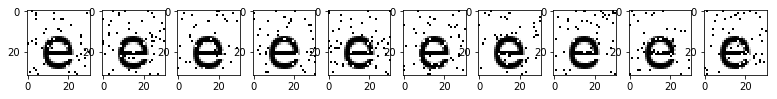
\includegraphics[width=\textwidth]{./images02/classification/low-noise-e.png}}

  \subfloat[Images from character ``f which were classified as {[i, f, f, I, I, I, f, f, f, f]}, respectively. It has made 4 misses. ]{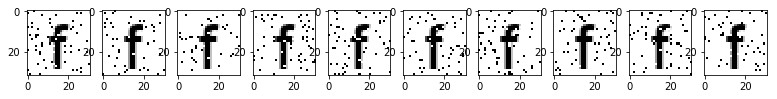
\includegraphics[width=\textwidth]{./images02/classification/low-noise-f.png}}

  \subfloat[Images from character ``l'' which were classified as {[i, i, i, i, i, i, i, i, i, i]}, respectively. It has missed them all, as if both groups have been merged. ]{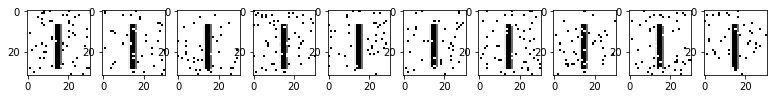
\includegraphics[width=\textwidth]{./images02/classification/low-noise-l.png}}

  \subfloat[Images from character ``t'' which were classified as {[t, t, t, t, t, t, t, i, t, t]}, respectively. It has made 1 miss. ]{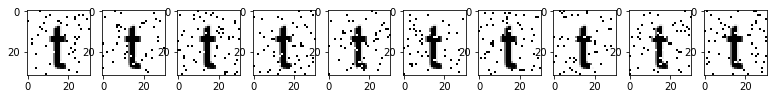
\includegraphics[width=\textwidth]{./images02/classification/low-noise-t.png}}

  \subfloat[Images from character ``9'' which were classified as {[9, 9, 0, 9, 9, 9, 0, 0, 9, 9]}, respectively. It has made 3 misses. ]{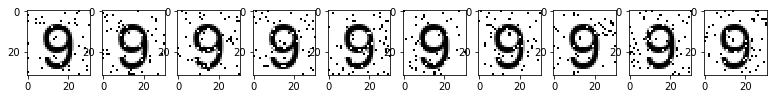
\includegraphics[width=\textwidth]{./images02/classification/low-noise-9.png}}

  \caption{Characters in the low noise scenario in which the classifier has made at least one mistake. In all the other cases, it correctly classified the images. We may notice that the groups of ``i'' and ``l'' have been completely merged by the classifier, because it cannot distinguish them, not even with no noise.}
  \label{fig-classification-low-noise-results}
\end{figure}

The high noise scenario is the most interesting, because, even in a high noise level, the classifier has hit most of the characters. It has hit all images for 44 out of 62 groups, and made at least one miss for the other 18 groups. The misses may be seen in details in Figure \ref{fig-classificiation-high-noise-misses}.

\begin{figure}[!htb]
  \centering
  \subfloat[Images from character ``B'' which were classified as {[S, B, B, B, B, B, B, B, B, B]}. It has made 1 mistake. ]{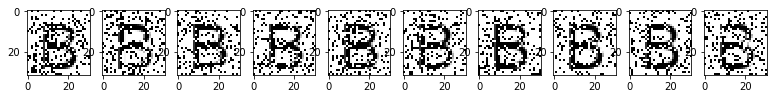
\includegraphics[width=\textwidth]{./images02/classification/high-noise-B.png}}

  \subfloat[Images from character ``O'' which were classified as {[G, G, O, O, O, O, O, O, O, O]}. It has made 2 mistakes. ]{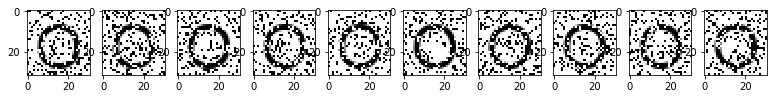
\includegraphics[width=\textwidth]{./images02/classification/high-noise-O.png}}

  \subfloat[Images from character ``T'' which were classified as {[T, T, T, T, T, I, T, T, T, T]}. It has made 1 mistake. ]{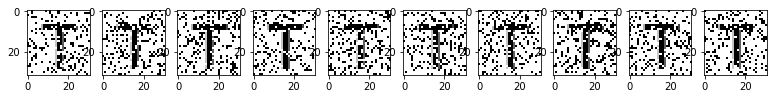
\includegraphics[width=\textwidth]{./images02/classification/high-noise-T.png}}

  \subfloat[Images from character ``Y'' which were classified as {[Y, I, Y, Y, Y, Y, Y, Y, Y, Y]}. It has made 1 mistake. ]{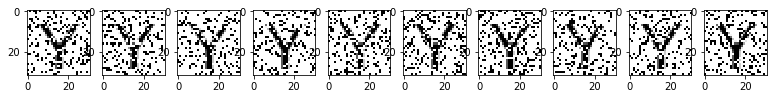
\includegraphics[width=\textwidth]{./images02/classification/high-noise-Y.png}}

  \subfloat[Images from character ``b'' which were classified as {[o, o, o, b, o, h, h, b, b, o]}. It has made 7 mistakes. ]{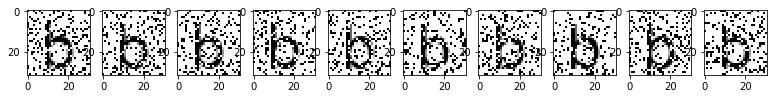
\includegraphics[width=\textwidth]{./images02/classification/high-noise-b2.png}}

  \subfloat[Images from character ``c'' which were classified as {[c, c, c, c, c, o, c, c, c, o]}. It has made 2 mistakes. ]{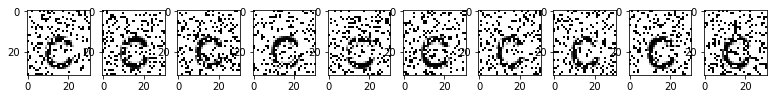
\includegraphics[width=\textwidth]{./images02/classification/high-noise-c.png}}

  \subfloat[Images from character ``e'' which were classified as {[e, o, e, o, o, o, e, o, o, e]}. It has made 6 mistakes. ]{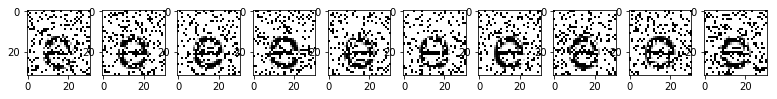
\includegraphics[width=\textwidth]{./images02/classification/high-noise-e.png}}

  \subfloat[Images from character ``f'' which were classified as {[I, I, I, I, i, I, I, I, I, I]}. It has missed them all. ]{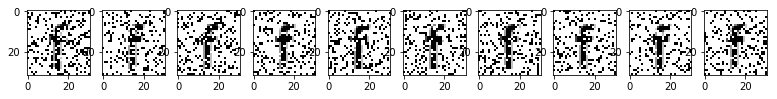
\includegraphics[width=\textwidth]{./images02/classification/high-noise-f.png}}

\end{figure}
\begin{figure}[!htb]\ContinuedFloat

  \subfloat[Images from character ``i'' which were classified as {[i, i, i, I, i, i, i, i, I, i]}. It has made 2 mistakes. ]{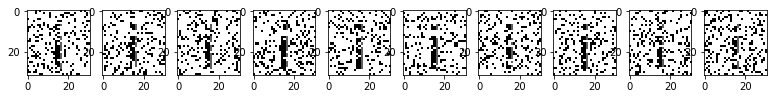
\includegraphics[width=\textwidth]{./images02/classification/high-noise-i.png}}

  \subfloat[Images from character ``j'' which were classified as {[j, j, j, I, I, j, j, j, j, I]}. It has made 3 mistakes. ]{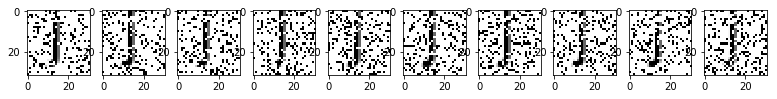
\includegraphics[width=\textwidth]{./images02/classification/high-noise-j.png}}

  \subfloat[Images from character ``l'' which were classified as {[I, i, I, I, I, I, i, I, I, i]}. It has missed them all. ]{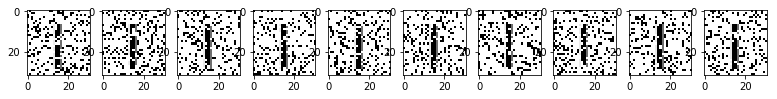
\includegraphics[width=\textwidth]{./images02/classification/high-noise-l.png}}

  \subfloat[Images from character ``n'' which were classified as {[u, n, n, n, n, n, u, u, u, h]}. It has made 5 mistakes. ]{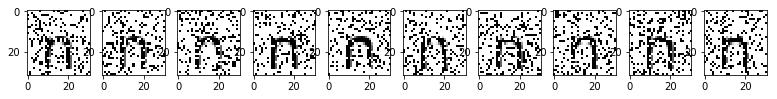
\includegraphics[width=\textwidth]{./images02/classification/high-noise-n.png}}

  \subfloat[Images from character ``q'' which were classified as {[q, q, q, q, q, q, q, q, q, g]}. It has made 1 mistake. ]{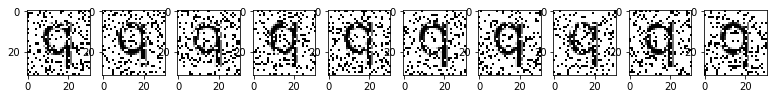
\includegraphics[width=\textwidth]{./images02/classification/high-noise-q.png}}

  \subfloat[Images from character ``t'' which were classified as {[I, r, I, i, I, i, i, i, I, i]}. It has missed them all. ]{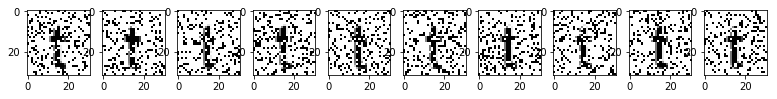
\includegraphics[width=\textwidth]{./images02/classification/high-noise-t2.png}}

  \subfloat[Images from character ``1'' which were classified as {[1, I, 1, I, 1, 1, I, I, 1, I]}. It has made 5 mistakes. ]{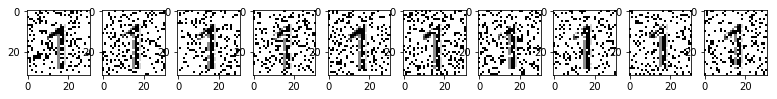
\includegraphics[width=\textwidth]{./images02/classification/high-noise-1.png}}

  \subfloat[Images from character ``7'' which were classified as {[7, 7, 7, I, 7, I, I, 7, 7, 7]}. It has made 3 mistakes. ]{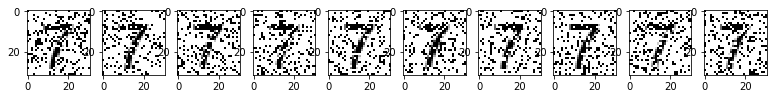
\includegraphics[width=\textwidth]{./images02/classification/high-noise-7.png}}

\end{figure}
\begin{figure}[!htb]\ContinuedFloat

  \subfloat[Images from character ``8'' which were classified as {[8, 6, 6, 6, 8, d, 8, 8, d, 6]}. It has made 6 mistakes. ]{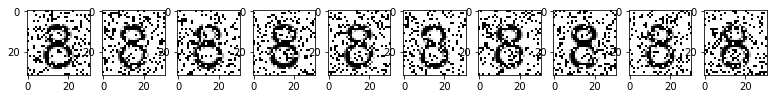
\includegraphics[width=\textwidth]{./images02/classification/high-noise-8.png}}

  \subfloat[Images from character ``9'' which were classified as {[9, 0, 6, 0, 9, 0, 0, 9, 0, 0]}. It has made 7 mistakes. ]{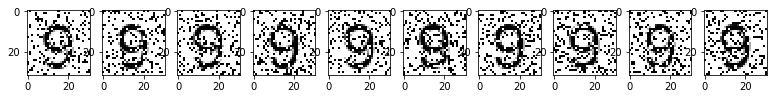
\includegraphics[width=\textwidth]{./images02/classification/high-noise-9.png}}

  \caption{Characters in the high noise scenario in which the classifier has made at least one mistake. In all the other cases, it correctly classified the images.}
  \label{fig-classification-high-noise-misses}
\end{figure}

The critical distance plays an important role in the classification error. As we have 62 groups and each have been trained with 100 images, there were 6,200 writes to the memory. When an image is being classified, it will have to converge to a group, and the convergence depends on the distance between this image and the images from the training set, i.e, in the noise level.

These results show that the SDM may be used as a supervised classification algorithm. Although we do not believe that the mapping between images and bitstrings are even close to the way human cognition deals with images, we believe the results are interesting and useful to many possible real world problems.


\chapter{Results (vi): Supervised image noise filtering application}

Image noise filtering consists in removing the noise from an input, in out case an image. Our images are black \& white images and the noise is generated randomly flipping some of their pixels from black to while and vice versa. In Figure \ref{fig-filter-progressive-noise}, we may see an image with different levels of noise, from 0\% to 45\% in steps of 5\%. It makes no sense to apply 50\% of noise because it would absolutely randomize the image.

\begin{figure}[!htb]
\centering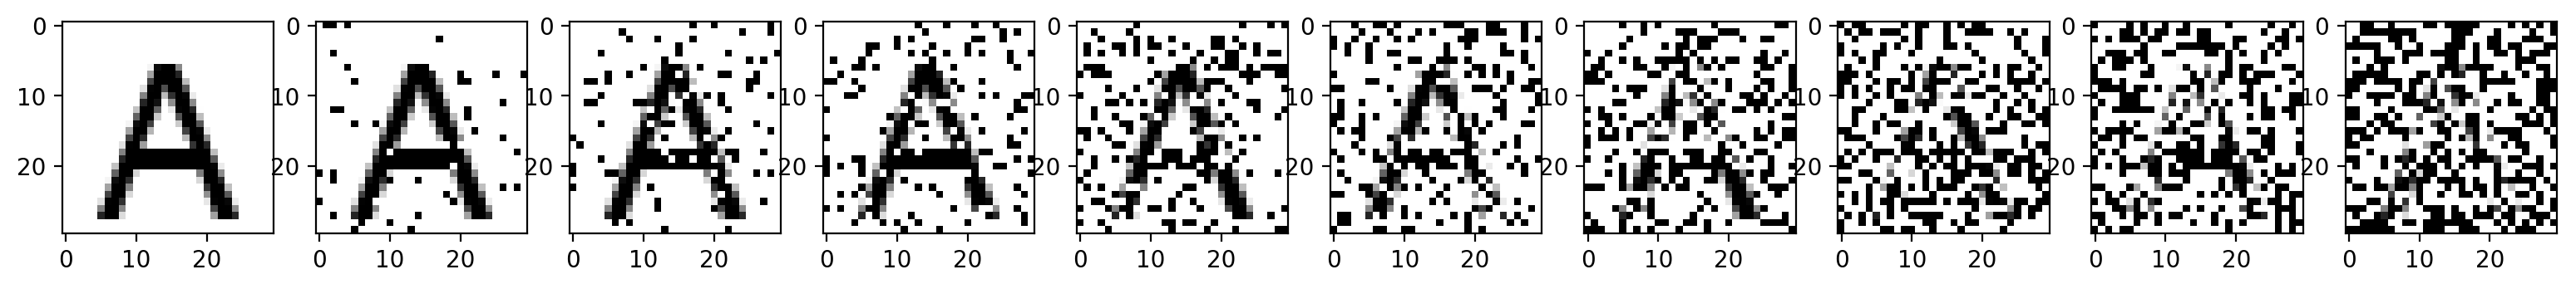
\includegraphics[width=\textwidth]{./images02/filter/progressive-noise.png}
\caption{Progressive noise into letter ``A'', from 0\% to 45\% in steps of 5\%.
\label{fig-filter-progressive-noise}}
\end{figure}

The images have 30 x 30 pixels, totaling 900 pixels per image. Each image is mapped into a 1,000 bit bitstring in which the bits are set according to the color of each pixel of the image. White pixels are equal to bit 0, and black pixels to bit 1. The 100 remaining bits are all set to zero. This is a bijective mapping (or one-to-one) from images and bitstrings, i.e., there is one, and only one, bitstring for each image, and vice versa.

In the learning phase, noisy images are generated and they are written into SDM chunked with their labels. The chunk was calculated using the exclusive or (XOR) operator. So, the image bitstring was written to the address of its bitstrings XOR its label bitstring --- write(addr=bs\_image XOR bs\_label, datum=bs\_image).

Finally, in order to remove the noise of a new image, first we have to classify it (possibly using the already presented classification algorithm), and then we just have to read from the chunked address until it converges.



\chapter{Results (vii): The possibility of unsupervised reinforcement learning}

Reinforcement learning has increasing prominence in the media after AlphaZero has won all games from both the best chess grandmasters in the world and the best chess engines. What is incredible about these victories is that AlphaZero has almost no knowledge about chess game and has learned all its movement playing against itself for 4 hours. Basically, it knowns only the valid movements and had to learn everything from scratch, which it did using a reinforcement learning algorithm.

Reinforcement learning is a machine learning algorithm which learns from the rewards of its actions. So, it receives the game state as input, then it decides which action will be taken, and finally it learns from the rewards of all the actions it has chosen. In theory, it learns after each reward feedback it receives, improving its decision over time and presenting intelligent behavior. A positive reward would indicate that the chosen action should be encouraged. While a negative reward would indicate the opposite. In some algorithms, there may be a neutral reward which would indicate that the chosen action was neither positive nor negative. How each type of reward should be handled depends on each algorithm.

We have done some experiments with an SDM as a memory for a TicTacToe player. Basically, it receives the current board state and returns which action should be played. In the end of the game, it receives the sequences of boards and the winner, and is supposed to learn from them.

Our algorithm to decide what should be player is very simples: it read the current board from SDM. If the reading converges to another board, it chooses the movement which would bring the current board to the one read from SDM. If the reading does not converge, it just play randomly.

After a game has finished, it is time to learn from its decisions. Thus, if SDM wins the game, it will write the whole sequence of boards to SDM. Let $b_0, b_1, b_2, \dots, b_n$ be the board sequence of the game (see Figure \ref{fig-ttt-example}). Then it will write $b_0 \rightarrow b_1 \rightarrow b_2 \rightarrow \cdots \rightarrow b_n$, with possibly different weights for each transition. If it loses, it will reverse the board (replace X by O and vice versa), and will act as if it had won. Hence, it will learn which sequences lead to victory. When a new board appears, it may have already seen that situation and will decide according to the sequences which goes towards victory. This is our positive reward learning.

\begin{figure}
    \captionsetup[subfigure]{labelformat=empty}
    %\centering

    \subfloat[$b0$]{\begin{tabular}{p{\widthof{x}}|p{\widthof{x}}|p{\widthof{x}}}
     & & \\\hline  & & \\\hline  & &
    \end{tabular}}
    {$\xrightarrow{w_0}$}
    \subfloat[$b1$]{\begin{tabular}{p{\widthof{x}}|p{\widthof{x}}|p{\widthof{x}}}
     & & \\\hline  &x& \\\hline  & &
    \end{tabular}}
    {$\xrightarrow{w_1}$}
    \subfloat[$b2$]{\begin{tabular}{p{\widthof{x}}|p{\widthof{x}}|p{\widthof{x}}}
     & & \\\hline o&x& \\\hline  & &
    \end{tabular}}
    {$\xrightarrow{w_2}$}
    \subfloat[$b3$]{\begin{tabular}{p{\widthof{x}}|p{\widthof{x}}|p{\widthof{x}}}
    x& & \\\hline o&x& \\\hline  & &
    \end{tabular}}
    {$\xrightarrow{w_3}$}
    \subfloat[$b4$]{\begin{tabular}{p{\widthof{x}}|p{\widthof{x}}|p{\widthof{x}}}
    x& & \\\hline o&x& \\\hline  & &o
    \end{tabular}}
    {$\xrightarrow{w_4}$}
    \subfloat[$b5$]{\begin{tabular}{p{\widthof{x}}|p{\widthof{x}}|p{\widthof{x}}}
    x&x& \\\hline o&x& \\\hline  & &o
    \end{tabular}}
    {$\xrightarrow{w_5}$}
    \subfloat[$b6$]{\begin{tabular}{p{\widthof{x}}|p{\widthof{x}}|p{\widthof{x}}}
    x&x&o\\\hline o&x& \\\hline  & &o
    \end{tabular}}
    {$\xrightarrow{w_6}$}
    \subfloat[$b7$]{\begin{tabular}{p{\widthof{x}}|p{\widthof{x}}|p{\widthof{x}}}
    x&x&o\\\hline o&x& \\\hline  &x&o
    \end{tabular}}

    \caption{Example of a game with 7 movements in which X wins.\label{fig-ttt-example}}
\end{figure}

It is also important to learn when a draw happens --- after all, it is better to tie than to lose, right? In this case, the sequence of boards is also written to SDM, but with no weight at all. So, if the board has appeared both in a tie sequence and in a winning sequence, it would be more likely to choose the winning one because it was written with greater weight. This is our neutral reward learning.

Finally, we also want to prevent losing games. So, when it loses a game, it will stimulate movements different from the chosen ones. Thus, for each transition $b_k \rightarrow b_{k+1}$ made by its action, it will write all possible transitions from $b_k$ but $b_{k+1}$.

Internally, every board is mapped into a random bitstring and passed to SDM. Thus, SDM knows nothing about the boards themselves. It knowns only about their transition and which ones would lead to either a victory or a draw. As every two boards are orthogonal, SDM does not known whether two boards are consecutives or not. The only link between two boards is the transition written in SDM.

After all, SDM knowns nothing about the boards themselves and yet it may learn how to play TicTacToe.

In order to properly run the discussed algorithms, it is necessary to have two SDMs: a 0-fold and a 1-fold SDM. In the 0-fold SDM, every bitstring is written to its own address. In the 1-fold SDM, every bitstring points to another one. So, the transitions are written in the 1-fold SDM, while the boards themselves are written to the 0-fold SDM. The boards are written only once in the 0-fold, no matter how many times they appear. The transitions may be written more than once in the 1-fold SDM, because it would reinforce that transition.

In more details, the next movement decision consists in one read from the 1-fold SDM, resulting in a bitstring. Then this bitstring is used in an interative reading from the 0-fold SDM, which will converge to the bitstring associated with the next board. If it does not converge to any board, than SDM will choose a random movement and learn from it. Eventually it may converge to a board which is not a sequence of the current board. In this case, SDM will also choose a random movement.

The weight used when writing a winning sequence is calculated using ...

--- talk about player generations ---

\subsection{Training}

It is an unsupervised algorithm because SDM learns playing against an opponent, who may be another SDM player, a human, or a player whose movements are always random.

Thus, in order to train a SDM player, we just have to keep it playing over and over.


\subsection{Results}



\begin{forest}
  TTT/.style args={#1:#2}{
    make tab/.expanded=\forestove{content},
    label={\pgfkeysvalueof{/forest/label position #1}:$#2$}
  },
  TTT*/.style={
    make tab=::/::/::,
    content/.expand once=%
    \expandafter\vphantom\expandafter{\romannumeral-`0\forestov{content}},
    draw=none,
    append after command={(\tikzlastnode.north) edge (\tikzlastnode.south)},
    for descendants={before computing xy={l*=1.2}},
  },
  th/.style=thick,
  for tree={node options=draw, inner sep=+0pt, parent anchor=south, child anchor=north}
%
[::/::/::, TTT=r:1
  [x::/::/::, TTT=r:-1
    [x::/::/::, TTT=r:-1
      [x::/::/::, TTT=r:-1
      ]
    ]
  ]
]
\end{forest}

\subsection{Results}
